\documentclass{article}
\usepackage{natbib}
\usepackage{amssymb, amsmath, amsfonts}
\usepackage{graphicx}
% ------------------------------------------------------------------------
% Packages
% ------------------------------------------------------------------------
\usepackage{amsmath}

% ------------------------------------------------------------------------
% Macros
% ------------------------------------------------------------------------
%~~~~~~~~~~~~~~~
% List shorthand
%~~~~~~~~~~~~~~~
\newcommand{\BIT}{\begin{itemize}}
\newcommand{\EIT}{\end{itemize}}
\newcommand{\BNUM}{\begin{enumerate}}
\newcommand{\ENUM}{\end{enumerate}}
%~~~~~~~~~~~~~~~
% Text with quads around it
%~~~~~~~~~~~~~~~
\newcommand{\qtext}[1]{\quad\text{#1}\quad}
%~~~~~~~~~~~~~~~
% Shorthand for math formatting
%~~~~~~~~~~~~~~~
\newcommand\mbb[1]{\mathbb{#1}}
\newcommand\mbf[1]{\mathbf{#1}}
\def\mc#1{\mathcal{#1}}
\def\mrm#1{\mathrm{#1}}
%~~~~~~~~~~~~~~~
% Common sets
%~~~~~~~~~~~~~~~
\def\reals{\mathbb{R}} % Real number symbol
\def\integers{\mathbb{Z}} % Integer symbol
\def\rationals{\mathbb{Q}} % Rational numbers
\def\naturals{\mathbb{N}} % Natural numbers
\def\complex{\mathbb{C}} % Complex numbers
\def\simplex{\mathcal{S}} % Simplex
%~~~~~~~~~~~~~~~
% Common functions
%~~~~~~~~~~~~~~~
\renewcommand{\exp}[1]{\operatorname{exp}\left(#1\right)} % Exponential
\def\indic#1{\mbb{I}\left({#1}\right)} % Indicator function
\providecommand{\maximize}{\mathop\mathrm{maximize}} % Defining math symbols
\providecommand{\maximize}{\mathop\mathrm{minimize}}
\providecommand{\argmax}{\mathop\mathrm{arg max}}
\providecommand{\argmin}{\mathop\mathrm{arg min}}
\providecommand{\arccos}{\mathop\mathrm{arccos}}
\providecommand{\asinh}{\mathop\mathrm{asinh}}
\providecommand{\dom}{\mathop\mathrm{dom}} % Domain
\providecommand{\range}{\mathop\mathrm{range}} % Range
\providecommand{\diag}{\mathop\mathrm{diag}}
\providecommand{\tr}{\mathop\mathrm{tr}}
\providecommand{\abs}{\mathop\mathrm{abs}}
\providecommand{\card}{\mathop\mathrm{card}}
\providecommand{\sign}{\mathop\mathrm{sign}}
\def\rank#1{\mathrm{rank}({#1})}
\def\supp#1{\mathrm{supp}({#1})}
%~~~~~~~~~~~~~~~
% Common probability symbols
%~~~~~~~~~~~~~~~
\def\E{\mathbb{E}} % Expectation symbol
\def\Earg#1{\E\left[{#1}\right]}
\def\Esubarg#1#2{\E_{#1}\left[{#2}\right]}
\def\P{\mathbb{P}} % Probability symbol
\def\Parg#1{\P\left({#1}\right)}
\def\Psubarg#1#2{\P_{#1}\left[{#2}\right]}
\def\Cov{\mrm{Cov}} % Covariance symbol
\def\Corr{\mrm{Corr}} % Covariance symbol
\def\Covarg#1{\Cov\left[{#1}\right]}
\def\Covsubarg#1#2{\Cov_{#1}\left[{#2}\right]}
\def\Corrsubarg#1#2{\Corr_{#1}\left[{#2}\right]}
\def\Var{\mrm{Var}}
\def\Vararg#1{\Var\left(#1\right)}
\def\Varsubarg#1#2{\Var_{#1}\left(#2\right)}
\newcommand{\family}{\mathcal{P}} % probability family
\newcommand{\eps}{\epsilon}
\def\absarg#1{\left|#1\right|}
\def\msarg#1{\left(#1\right)^{2}}
\def\logarg#1{\log\left(#1\right)}
%~~~~~~~~~~~~~~~
% Distributions
%~~~~~~~~~~~~~~~
\def\Gsn{\mathcal{N}}
\def\Ber{\textnormal{Ber}}
\def\Bin{\textnormal{Bin}}
\def\Unif{\textnormal{Unif}}
\def\Mult{\textnormal{Mult}}
\def\Cat{\textnormal{Cat}}
\def\Gam{\textnormal{Gam}}
\def\InvGam{\textnormal{InvGam}}
\def\NegMult{\textnormal{NegMult}}
\def\Dir{\textnormal{Dir}}
\def\Lap{\textnormal{Laplace}}
\def\Bet{\textnormal{Beta}}
\def\Poi{\textnormal{Poi}}
\def\HypGeo{\textnormal{HypGeo}}
\def\GEM{\textnormal{GEM}}
\def\BP{\textnormal{BP}}
\def\DP{\textnormal{DP}}
\def\BeP{\textnormal{BeP}}
%~~~~~~~~~~~~~~~
% Theorem-like environments
%~~~~~~~~~~~~~~~

%-----------------------
% Probability sets
%-----------------------
\newcommand{\X}{\mathcal{X}}
\newcommand{\Y}{\mathcal{Y}}
\newcommand{\D}{\mathcal{D}}
\newcommand{\Scal}{\mathcal{S}}
%-----------------------
% vector notation
%-----------------------
\newcommand{\bx}{\mathbf{x}}
\newcommand{\by}{\mathbf{y}}
\newcommand{\bt}{\mathbf{t}}
\newcommand{\xbar}{\overline{x}}
\newcommand{\Xbar}{\overline{X}}
\newcommand{\tolaw}{\xrightarrow{\mathcal{L}}}
\newcommand{\toprob}{\xrightarrow{\mathbb{P}}}
\newcommand{\laweq}{\overset{\mathcal{L}}{=}}
\newcommand{\F}{\mathcal{F}}


\title{Multitable Data Analysis for the Microbiome}
\author{Kris Sankaran}

\begin{document}
\maketitle

The simultaneous study of multiple measurement types is a commonly encoutered
problem in practical data analysis. It is especially common in microbiome
research, where several sources of data -- for example, 16s, metagenomic,
metabolomic, or transcriptomic data -- can be collected on the same physical
samples\citep{Franzosa2015, McHardy2013}. There has been a proliferation of
proposals for analyzing this kind of data, as is often the case when new (or
more cheaply available) data sources makes inquiry into certain scientific
questions all of a sudden possible \citep{Fukuyama2017, Rahnavard2017,
  Chaudhary2017, Chalise2017}.

However, stepping back from the rush of new methods for multiple table analysis
in the microbiome literature, it is worthwhile to recognize the broader
landscape of multiple table methods, as they have been relevant in problem
domains ranging from economics to robotics to computational biology. Of course,
there is no unique optimal algorithm to use across domains -- different
instances of the multiple table problem possess specific structure or variation
that are worth incorporating in methodology.

Our purpose here is not to develop new algorithms, but rather to (1) distill the
relevant themes across different analysis approaches and (2) provide concrete
workflows for approaching analysis, as a function of ultimate analysis goals and
characteristics (heterogeneity, dimensionality, sparsity, ...) of the data.
Towards the second goal, code for all analysis and figures are available.

First, though, why does anyone bother collecting multiple sources of data, and
why can't these sources simply be combined into a single, unified table for
subsequent analysis? One answer is simply that it's now cheaper and easier to
collect multitable data, but a more satisfactory explanation is that many
scientific problems can only be answered by collecting several complementary
measurement types. Indeed, the situation is analogous to using many types of
sensors to study a single system from many perspectives. Further, while in
certain supervised problems, it is enough to predict a single measurement of
interest, with other sources simply collected to provide better features, there
are often an additional relational components to the analysis: how do different
types of measurements covary with one another? Here, it is of interest to
provide a reduction / representation of the data that facilitates comparisons
across tables, rather than just comparing each table with a single response of
interest. This richer scientific question motivates the development of methods
distinct from those used to analyze a single measurement type at a time.

For more concrete motivation, we will use data from the WELL-China study, which
is focused on the relationship between various indicators of wellness and
microbial community structure (todo: give reference). In this study, 1969
individuals\footnote{Though sampling is still ongoing.} underwent clinical
examinations, filled out wellness surveys (covering topics such as exercise,
sleep, diet, and mental health, for example), and provided stool samples, used
for 16s sequencing and metabolomic analysis. To date, 16s sequencing data is
available for 221 of these participants. Evidently, various interesting
relational questions can be investigated using this data source.

For the purpose of illustration, we focus on one relatively focu
sed question
that can be addressed using this data: How is the distribution of lean and fat
mass across the body related to patterns of microbial abundance? The measurement
types most relevant in this analysis are (1) DEXA scans and (2) 16s sequencing.
DEXA scans use relative X-ray absorption to gauge the among of lean and fat body
mass within the region of the body being scanned. We will have access to these
lean and fat body mass measurements at several body sites -- arms, legs, trunk,
etc. -- along with related body type variables, like height, age, and android
and gynoid fat measurements. In total, there are 33 of these variables. 16s
sequencing is a technology for gauging the abundance of differnet bacterial
species in the gut by counting the alignments of reads to the 16s gene, a
component of all bacterial genomes with enough variation to allow discimination
between different individual species. We have counts associated with 2565
species across 181 genuses, though the vast majority are present in low
abundances.

This question of the relationship between lean and fat mass distribution
(informally, body type) and the microbiome follows up findings that certain
taxonomic groups are over or underrepresented as a function of an individual's
BMI or obesity \citep{ley2006microbial, turnbaugh2009core, ley2005obesity,
  ley2010obesity}. Further, since the distribution of fat is often more related
to underlying biological mechanisms than overall body mass
\citep{matsuzawa2008role}, and since this distribution is mediated by specific
metabolic pathways, there is reason to suspect that a joint analysis of DEXA and
16s microbial abundance data might yield a more complete view of the
relationship between the microbiome and body type (and the associated disease
risk factors).

\section{Classical multivariate methods}

Methods from classical multivariate statistics are a mainstay of single-table
microbiome data analysis, so it is natural to revisit this literature before
surveying extensions to the multitable setting. Here we describe a few of the
classically studied multitable methods that fit nicely into the modern
microbiome data analysis toolbox. We first describe a naive approach based on
Principal Components Analysis (PCA) -- naive because it lifts a single-table
method to the multiple table setting without any special considerations --
before studying approaches that directly characterize covariation across several
tables: Canonical Correlation Analysis (CCA), Multiple Factor Analysis (MFA),
and Principal Component Analysis with Instrumental Variables (PCA-IV).

The earliest multitable method (CCA) was published in 1936, where the motivating
data analysis problem was to relate prices of groups of commodities
\citep{hotelling1936relations}. There are two notable aspects of data analysis in
this classical paradigm which no longer hold in modern statistics:
\begin{itemize}
  \item Even when many samples could be collected, there were typically only a
    few features for each sample, and it was straightforwards to study all of
    them simultaneously. In the last few decades, it has become possible to
    automatically collect a large number of features for each sample.
  \item Before electronic computers had been invented, it was important that all
    statistical quantities be easy to calculate, typically necessitating
    analytical formulas for parameter estimates. This is no longer as important
    a limitation in an environment with richer computational resources.
\end{itemize}

These changes have motivated the need for high-dimensional methods and
facilitated the adoption of iterative, more computationally-intensive
approaches, respectively, some of which are described later in this review.

Nonetheless, it is worth reviewing these original approaches, both to understand
the context for many modern techniques, as well as to have an easy starting
point for practical data analysis. Indeed, these more established methods tend
to be the most readily available through statistical computing packages and can
provide a benchmark with which to compare more elaborate, modern methods.

\subsection{PCA}
\label{subsec:pca}

The simplest approach to dealing with multiple tables is to combine them into
one and apply a single-table method, for example, PCA. That is, write
\begin{align*}
X = \left[X^{(1)} \vert \dots \vert X^{(L)}\right] \in \reals^{n \times p},
\end{align*}
where $p = \sum_{l = 1}^{L}p_{l}$, and compute the SVD\footnote{An equivalent
  procedure is to eigenanalyze the empirical covariance matrix
  $\frac{1}{n}X^{T}X$.}, $X = UDV^{T}$. The $K$-principal component directions
are the first $K$ columns $v_{\cdot 1}, \dots, v_{\cdot K}$, while the
associated scores are $d_{1}u_{\cdot 1}, \dots, d_{K}u_{\cdot K}$.

While this does not account for the multitable structure of the data, it does
accomplish two goals,
\begin{itemize}
\item Through the principal component scores, it provides a visualization of the
  relationships between samples, based on all features.
\item Through the principal component directions, it gives a way of relating
  features within and across the multiple tables.
\end{itemize}

However, two drawbacks of this approach are worth noting,
\begin{itemize}
  \item It does not provide a summary of the relationship between the sets of
    variables defining the tables -- it can only relate pairs of
    variables. \label{bullet:pca_drawback_one}
  \item If some tables have many more variables than others, they can dominate
    the resulting ordination. \label{bullet:pca_drawback_two}
\end{itemize}

These limitations are addressed by CCA and MFA, discussed in Sections
\ref{subsec:cca} and \ref{subsec:mfa}, respectively.

Here we describe one geometric and one statistical motivation for PCA. The
geometric motivation is that, if each row $x_{i}$ of $X$ is viewed as a point in
$p$-dimensional space, then the principal component directions provide the best
$k$-dimensional approximation to the data, see Figure \ref{fig:pca-approx}.
Formally, recall that $VV^{T}x_{i}$ is the projection of $x_{i}$ onto the
subspace spanned by the columns of $V$. PCA identifies the orthogonal matrix $V
\in \reals^{p \times K}$ such that
\begin{align*}
\sum_{i = 1}^{n}\|x_{i} - VV^{T} x_{i}\|_{2}^{2}
\end{align*}
is minimized. The principal component scores are then the coordinates of the
projected points with respect to this subspace.

\begin{figure}
  \includegraphics[width=0.7\textwidth]{figure/pca/proj_plot_1}
  \caption{A geometric motivation for PCA. The first principal component spans
    the one-dimensional subspace $V$ minimizing the squared error between points
    and their projections, $\sum_{i = 1}^{n}\|\left(I -
    VV^{T}\right)x_{i}\|_{2}^{2}$ projections. The black points represent the
    scaled values for two of the body composition variables --  and total
    fat mass -- while the purple points are the projections onto the first
    principal component when only accounting for these two variables. Contrast
    this with Figures \ref{fig:pca-approx-2} and \ref{fig:pca-approx-3}, where
    variables other than  and fat mass are taken into account.}
  \label{fig:pca-approx}
\end{figure}

\begin{figure}
  \includegraphics[width=\textwidth]{figure/pca/var_plot}
  \caption{A statistical motivation for PCA. Each histogram is computed from the
    linear combinations $\left(c^{j}x_{i}\right)$, for $c^{j}$ equal to the
    first and second principal components, the vector $\frac{1}{n}\mathbf{1}$,
    and a normalized random multivariate Gaussian. At least among these four
    vectors, the scores obtained from the first PC have the largest variance. It
    is a theorem that its variance is in fact maximal among all linear
    combinations with orthogonal vectors.}
  \label{fig:pca-var}
\end{figure}

The second interpretation is that PCA finds a low-dimensional representation of
the $x_{i}$ such that the resulting points have maximal variance. Qualitatively,
this is a desirable property, because it means that the simpler representation
preserves most of the variation present in the original data, see Figure
\ref{fig:pca-var}. In this figure, histograms of the scores associated with four
linear combinations of the original body composition measurements are displayed
side by side, to emphasize the fact that the linear combination $x^{T}v_{1}$
associated with the first principal component $v_{1}$ has the largest variance.
The comparison combinations are the second principal component, the mean across
all columns, and a random linear combination $\frac{c^{T}}{\|c\|} x$ where $c \sim
\Gsn\left(0, I_{p}\right)$.

Formally, suppose that the $x_{i}\in\reals^{p}$ are drawn
independently from some distribution $\P$, so that the variance is
$\Covsubarg{\P}{x_{i}} = \Sigma$. Consider an arbitrary linear combination of
$x_{i}$'s $p$ coordinates: $z_{i} := c^{T}x_{i}$ for some $c \in \reals^{p}$.
The first PCA direction gives the $c$ such that the variance of this coordinate,
$\Varsubarg{\P}{z_{i}} = c^{T}\Sigma c$, is maximal. The second direction gives
the linear combination that maximizes variance, subject to being orthogonal to
the first, and so forth.

While our description of the method of concatenating multiple tables into a
single one has focused on PCA, note that other methods could be applied instead.
For example, it is possible to define a new distance between samples as a
mixture of distances based on several tables. This can be useful if there are
different types of data across the different tables: Jaccard, $\chi^{2}$, and
euclidean distsances can be applied to binary, count, and real valued tables.
The combined distance can then be input into any distance-based single-table
procedure, like multidimensional scaling or hierarchical clustering. The primary
downside of this approach is that the resulting distance only allows a
comparison between samples, but not across features.

PCA is a very widely used technique, and some standard references include
\citep{friedman2001elements, mardia1980multivariate, pages2014multiple}.
Nonetheless, it is not ideal in the multitable setting. Its limitations prompt
us to begin our survey of multitable methods in earnest.

\subsubsection{Example}
\label{subsubsec:pca_example}

Figure \ref{fig:loadings} and \ref{fig:scores_total_fm} illustrate this approach
on body composition and bacterial abundance data from the WELL-China study.
Note that we have subsetted to only men, since men and women have very different
body compositions. Further, the 16s data have been variance stabilized according
the methodology proposed in \citep{Anders2010} and filtered to only those
amplicon sequence variants (ASVs) that are nonzero in at least 7\% of samples.

Figure \ref{fig:loadings} displays the loadings associated with this
combined-dataset PCA approach, where body composition (36 columns) and 16s
abundances (368 columns) were combined into one dataset (401 columns). Columns
associated with bacterial species are displayed as points, shaded by taxonomic
family, while columns associated with body composition variables are labeled
with text.

Most body composition variables lie on the top right, in a direction
approximately orthogonal to the main direction of variation among ASVs. Columns
that are highly correlated (e.g., right (R) and left (L) Trunk Fat Mass (FM)
have loadings nearly equal to one another. Age appears in generally negatively
correlated with the other, more  oriented, variables. Among ASVs, the main
source of variation seems to be between Ruminococcaceae and Lachnospiraceae,
which appear overrepresented on the left and right, respectively.

To identify relationships between ASVs and body composition variables, it would
be of interest to isolate those ASVs with large contributions along the axis
defined by linking the center of the  variables and the origin. Relatively
few such species stand out, though note that there is nothing in this
algorithm's objective that would seek covariation across tables directly, so the
fact that such associations seem weak with respect to the top two principal
components does not mean such relationships do not exist.

\begin{figure}[ht]
  \centering
  \includegraphics[width=\textwidth]{figure/pca/loadings}
  \caption{The loadings obtained by applying PCA to the combined body
    composition and microbial abundance data set. \label{fig:loadings} }
\end{figure}

We can study individual samples with respect to these loadings, by plotting
their projections onto the top two principal components. This is the content of
Figures \ref{fig:scores_total_fm} and \ref{fig:scores_rl_ratio}. These figures
display samples in the same positions, but shaded by  and Ruminococcaceae
/ Lachnospiraceae ratio, respectively. This shading confirms the observations
from the loadings directly using observed data. Indeed, the increasing
among samples in the top right of Figure \ref{fig:scores_total_fm} exactly
corresponds to the fact that  related variables lie in the top right in
Figure \ref{fig:loadings}. A left-to-right Ruminococcaceae /
Lachnospiraceae differentiation is visible in Figure \ref{fig:scores_rl_ratio},
which is consistent with the loadings, though we also observe a few samples with
substantially higher Ruminoccocus ratios.

In this approach, the loadings provide a description of the relationship between
variables across data sets. Further, scores summarize variation in samples
across multiple data sets. In this light, this simple heuristic is a natural
first step in analyzing multiple table data. However, considering the difficulty
in directly interpreting the covariation across data sets, as well as the
method's failure to use any sense of covariation in the dimensionality
reductions trategy, suggests that this method should not be the last step of an
analysis workflow. Nevertheless, we now have a baseline with which to compare
the more elaborate methods of subsequent sections.

\begin{figure}[ht]
  \centering
  \includegraphics[width=\textwidth]{figure/pca/scores_total_fm}
  \caption{The scores resulting from PCA applied to the combined body
    composition and microbial abundance data set.\label{fig:scores_total_fm} }
\end{figure}

\begin{figure}[ht]
  \centering
  \includegraphics[width=\textwidth]{figure/pca/scores_rl_ratio}
  \caption{The same scores as Figure \ref{fig:scores_total_fm}, but shaded now by
    the ratio of Ruminococcaceae over Lachnospiraceae relative abundances. The
    slight increase in Ruminococcaceae from left to right is consistent with the
    loadings observed in Figure \ref{fig:loadings}.\label{fig:scores_rl_ratio} }
\end{figure}

\subsection{CCA}
\label{subsec:cca}

CCA is a close relative of PCA that designed to compare sets of features across
tables. Like PCA, it provides low-dimensional representations of samples, but it
also allows comparisons at the table level. Suppose for now that there are only
two tables of interest, $X \in \reals^{n \times p_{1}}$ and $Y \in \reals^{n
  \times p_{2}}$. Let $\hat{\Sigma}_{XX}, \hat{\Sigma}_{YY}$, and
$\hat{\Sigma}_{XY}$ be the associated covariance estimates. Take the SVD,
$\hat{\Sigma}_{XX}^{-\frac{1}{2}}\hat{\Sigma}_{XY}\hat{\Sigma}_{YY}^{-\frac{1}{2}}
= \tilde{U}D\tilde{V}^{T}$. The canonical correlation directions associated with
the two tables are $u_{k} = \Sigma_{XX}^{-\frac{1}{2}}\tilde{u}_{k} \in
\reals^{p_{1}}$ and $v_{k} = \Sigma_{YY}^{-\frac{1}{2}}\tilde{v}_{k} \in
\reals^{p_{2}}$. These directions give two sets of low-dimensional
representations for each sample, one for each table: $z_{k}^{(1)} = Xu_{k} \in
\reals^{n}$ and $z_{k}^{(2)} = Yv_{k} \in \reals^{n}$. If the two tables are
closely related, then the $z_{k}^{(1)}$ and $z_{k}^{(2)}$ will be very
correlated. The singular values $d_{k}$ are called the canonical correlation
coefficients. Like the eigenvalues in PCA, they characterize the amount of
covariation across tables that can be captured by each additional pair of
directions.

As in PCA, there are many ways to view this procedure; here we discuss
geometric, statistical, and probabilistic interpretations. Unlike the geometric
interpretation for PCA, the geometric interpretation for CCA identifies point
locations with features, not samples. Specifically, the columns of $X$ and $Y$
are thought of as points in $\reals^{n}$. Consider two subspaces defined as the
spans of the columns of $X$ and $Y$, respectively. These subspaces correspond to
the linear combinations of features within each table. Place two ellipses on the
respective subspaces, centered at the origin and with size and shape depending
on the within table covariances $\hat{\Sigma}_{XX}$ and $\hat{\Sigma}_{YY}$. The
first canonical correlation directions are the pair of points, one lying on each
ellipse, such that the angle from the origin to those two points is smallest. In
this sense, it finds a pair of variance-constrained linear combinations of
features within the two tables so that the two combinations appear ``close'' to
one another. The second pair of canonical correlation directions identify a pair
of points with similar interpretation, except they are required to be orthogonal
to the first pair, with respect to the inner product induced by the covariances
in each table.

\begin{figure}[ht]
  \centering
  \includegraphics[width=0.8\textwidth]{figure/cca/geometric}
  \caption{The geometric representation of CCA, on a toy subset of the WELL-China
    data, to facilitate visualization. The three axes correspond correspond to
    three subjects, and the text labels indicate the positions of (scaled) features with
    respect to the samples. Features from the 16s table are shaded in blue,
    while body composition variables are orange. The subspaces spanned by the
    three features in each table are indicated by a grid of points lying along
    them, shaded in the same color as the measurement type they correspond to.
    We only display three features so that the table subspaces do are not simply
    all of $\reals^{3}$. A set of points lie along ellipses that are unit balls
    with respect to each data set's covariance matrix, estimated using all
    samples (not just the three displayed). Two arrows are the first CCA
    directions associated with the two measurement types. Evidently, the
    correlation between these measurement types, restricted to these few samples
    and features, is quite high, since the arrows point in nearly the same
    direction.
    \label{fig:cca_geometric} }
\end{figure}

For a statistical interpretation, the idea of CCA is to find the low-dimensional
representations of the two tables with maximal covariance -- this is analogous
to the maximum variance interpretation. Formally, let $x_{i}$ and $y_{i}$
samples from $\P^{\X}$ and $\P^{\Y}$. The rows of the two tables are imagined to
be i.i.d. draws from $\P^{\X\Y}$. Consider arbitrary linear combinations
$z_{i}^{(1)}\left(u\right) = u^{T} x_{i}$ and $z_{i}^{(2)}\left(v\right) =
v^{T}y_{i}$ of samples from the two tables. The first pair of CCA directions
$u_{1}^{\ast}$ and $v_{1}^{\ast}$ are chosen to optimize
\begin{align}
  \maximize_{u \in \reals^{p_{1}}, v \in \reals^{p_{2}}}
  &\Covsubarg{\P^{\X\Y}}{z_{i}^{(1)}\left(u\right),
    z_{i}^{(2)}\left(v\right)} \label{eq:cancor_optim} \\
\text{subject to } &\Varsubarg{\P^{\X}}{z_{i}^{(1)}\left(u\right)} = 1 \nonumber \\
&\Varsubarg{\P^{\Y}}{z_{i}^{(2)}\left(v\right)} = 1. \nonumber
\end{align}
To produce subsequent directions, the same optimization is performed, but with
the additional constraint that the directions must be orthogonal to all the
previous directions identified for that table. Of course, in actual
applications, we estimate these covariances and variances empirically.

This perspective makes it easy to derive the algorithm given at the start of
this section. The empirical version of the optimization problem
\ref{eq:cancor_optim} is
\begin{align}
  \maximize_{u \in \reals^{p_{1}}, v \in \reals^{p_{2}}}
  &u^{T}\hat{\Sigma}_{XY}v \label{eq:cancor_optim_emp}\\
  \text{subject to } & u^{T}\hat{\Sigma}_{XX}u = 1 \nonumber \\
  & v^{T}\hat{\Sigma}_{YY}v = 1. \nonumber
\end{align}

Consider the whitened data, $\tilde{u} = \hat{\Sigma}_{XX}^{\frac{1}{2}}u$ and
$\tilde{v} = \hat{\Sigma}_{YY}^{\frac{1}{2}}v$. The
optimization \label{eq:cancor_emp} can now be expressed as
\begin{align}
  \maximize_{\tilde{u} \in \reals^{p_{1}}, \tilde{v} \in
    \reals^{p_{2}} 
  &\tilde{u}^{T}\hat{\Sigma}_{XX}^{-\frac{1}{2}}\hat{\Sigma}_{XY}\hat{\Sigma}_{YY}^{-\frac{1}{2}}\tilde{v} \label{eq:cancor_trans} \\
\text{such that } & \|\tilde{u}\|^{2}_{2} = 1 \nonumber \\
&\|\tilde{v}\|_{2}^{2} = 1. \nonumber
\end{align}
The optimal $\hat{\tilde{u}}_1$ and $\hat{\tilde{v}}_1$ for this problem are
well known -- they're exactly the first left and right eigenvectors of
$\hat{\Sigma}_{XX}^{-\frac{1}{2}}\hat{\Sigma}_{XY}\hat{\Sigma}_{YY}^{-\frac{1}{2}}
= \tilde{U}D\tilde{V}^{T}$, respectively. The argument is standard\footnote{See
  \citep{mardia1980multivariate}, for example.}, but we include it for
completeness.

Let $\xi$ and $\nu$ be potential maximizers of length one. We can find $w_{u}$
and $w_{v}$ such that $\xi = \tilde{U}w_{u}, \nu = \tilde{V}w_{v}$, since
$\tilde{U}$ and $\tilde{V}$ are both orthonormal bases. Since they are length
one, $1 = \|\xi\|^{2}_{2} = w_{u}^{T}\tilde{U}^{T}\tilde{U}w_{u} =
\|w_{u}\|_{2}^{2}$ and similarly $\|w_{v}\|_{2}^{2} = 1$. The objective
\ref{eq:cancor_trans} can be bounded by
\begin{align*}
\xi^{T}\hat{\Sigma}_{XX}^{-\frac{1}{2}}\hat{\Sigma}_{XY}\hat{\Sigma}_{YY}^{-\frac{1}{2}}\nu
&= w_{u}^{T}\tilde{U}^{T}\tilde{U}D\tilde{V}^{T}\tilde{V}w_{v} \\
&= w_{u}^{T}Dw_{v} \\
&= \sum_{k = 1}^{p_{1} \wedge p_{2}} d_{k}w_{uk}w_{vk} \\
&\leq d_{1} \sum_{k = 1}^{p_{1} \wedge p_{2}} w_{uk}w_{vk} \\
&\leq d_{1} \|w_{u}\|\|w_{v}\| = d_{1},
\end{align*}
and this maximum is attained when $w_{u}$ and $w_{v}$ both put all their
on the first coordinate, that is $\xi = \tilde{u}_{1}$ and $\nu =
\tilde{v}_{1}$. For subsequent directions, we repeat the argument but require
that $w_{u}$ and $w_{v}$ have zero  on the first columns of $\tilde{U}$
and $\tilde{V}$.

To recover the solutions to the original problem, we reverse the original
variable transformation, yielding optimal $\hat{u}_{1} =
\Sigma_{XX}^{-\frac{1}{2}}\hat{\tilde{u}}_{1}$ and $\hat{v}_{1} =
\Sigma_{YY}^{-\frac{1}{2}}\hat{\tilde{v}}_{1}$.

A probabilistic interpretation of this procedure views it as estimating the
factors in an implicit latent variable model. In particular,
\citep{bach2005probabilistic} supposes that $x_{i}$ and $y_{i}$ are drawn i.i.d.
from the model,
\begin{align*}
  \xi_{i} := \left(\xi_{i}^{s}, \xi_{i}^{X}, \xi_{i}^{Y}\right) &\sim
  \Gsn\left(0, I_{d}\right) \\
  x_{i} \vert \xi_{i} &\sim \Gsn\left(W_{X}\xi_{i}^{s} + B_{X}\xi_{i}^{X} + \mu_{X},
  I_{d} \right) \\
  y_{i} \vert \xi_{i} &\sim \Gsn\left(W_{Y}\xi_{i}^{s} +
  B_{Y}\xi_{i}^{Y} + \mu_{Y}, I_{d}\right)
\end{align*}
That is, each sample is associated with a $d$-dimensional latent variable
$\xi_{i}$, drawn from a spherical normal prior. A few of the coordinates of
these latent variables contribute to shared structure, through $W_{X}$ and
$W_{Y}$. The remaining coordinates model table-specific structure, through
$B_{X}$ and $B_{Y}$. It can be shown that the posterior expectations of the
latent $\xi_{i}^{s}$ (assumed $\in \reals^{K}$) given the observed tables must
lie on the subspace defined by the CCA directions. More precisely,
\begin{align*}
  \Earg{\xi_{i} \mid x_{i}^{(1)}} \in \text{span}\left(z_{1}^{(1)},
    \dots, z_{K}^{(1)}\right),
\end{align*}
and
\begin{align*}
  \Earg{\xi_{i} \mid x_{i}^{(2)}} \in \text{span}\left(z_{1}^{(2)},
    \dots, z_{K}^{(2)}\right).
\end{align*}

Finally, we observe that the logic for CCA generalizes to an arbitrary number
$L$ of tables, by summing all pairwise covariances. That is, the instead of
finding directions $c_{k}^{(1)}$ and $c_{k}^{(2)}$ maximizing
$\Covsubarg{\P^{(1)}, \P^{(2)}}{c_{k}^{(1)T}x_{i}^{(1)},
  c_{k}^{(2)T}x_{i}^{(2)}}$ subject to normalization and orthogonality
constraints, we seek directions $c_{k}^{(1)}, \dots, c_{k}^{(L)}$ that maximize
the sum of cross-covariances $\sum_{l,l^{\prime} = 1}^{L} \Covsubarg{\P^{(l)},
  \P^{(l^{\prime})}}{c_{k}^{(l) T}x_{i}^{(l)},
  c_{k}^{(l^{\prime})}x_{i}^{(l^{\prime})}}$.

\subsubsection{Example}
\label{subsubsec:cca_example}

We next apply CCA to the WELL-China body composition and microbiome data sets,
with particular interest in how results compare with those of
Section \ref{subsubsec:pca_example}. To this end, we provide analogous loading and score
plots in Figures \ref{fig:cca_loadings} through \ref{fig:cca_scores_rl_ratio}.
However, note that the data are \textit{not} quite the same between the two
analysis -- we have filtered down to sequence passing a filter\footnote{Presence
  in at least half of samples}, which reduces the number of sequences to 57,
from 2565. This very aggressive filtering is necessary because CCA requires
estimation of covariances matrices $\Sigma_{XX}, \Sigma_{XY}$, and
$\Sigma_{YY}$, which is impossible for $p > n$ and highly unstable when $p$ a
large fraction of $n$. Besides this stronger filtering, all preprocessing steps
remain the same as in Section \ref{subsubsec:pca_example}.

\begin{figure}[ht]
  \centering
  \includegraphics[width=\textwidth]{figure/CCA/loadings}
  \caption{The loadings obtained by applying CCA to the combined body
    composition and microbial abundance data set. \label{fig:cca_loadings} }
\end{figure}

Figure \ref{fig:cca_loadings} provides the analog of CCA loadings. To be
precise, let $X \in \reals^{102\times 33}$ be the matrix of body composition
measurements and $Y \in \reals^{102 \times 57}$ be the variance stabilized
microbial abundances. As before, write $\hat{u}_{k} \in \reals^{33}, \hat{v}_{k}
\in \reals^{57}$ for the $k^{th}$ canonical correlation directions. Then, Figure
\ref{fig:cca_loadings} displays text labels for column $j$ of the body
composition variables at location $\times \left(u_{j1}, u_{j2}\right)_{j =
  1}^{33}$ and shaded points for the $j^{th}$ species at position
$\left(\hat{v}_{j1}, \hat{v}_{j2}\right)_{j = 1}^{57}$.

As in the joint PCA, we find that the groups of variables occupy separates
spaces. Our interpretation is that sequences further to the left are correlated
with the body variables further to the left, which are all in some ay variants
of . Note that age is negatively correlated with total fat mass, which is why it
appears on the opposite end. Among the abundant species that remain, there is
limited clustering according to taxonomic group, though the Bacteroideceae and
Ruminoccocus do appear restricted to the bottom and top right, respectively.
Note that the third CCA axis (the size of plotted text and points) distinguishes
lean and fat mass variables.

In Figure \ref{fig:cca_scores_linked} we plot the corresponding scores. Note
that in CCA, there are two sets of scores for each $k$, the $X\hat{u}_{k}$ and
$Y\hat{v}_{k}$. Indeed, the CCA objective finds directions that maximizes the
correlation between these scores. In this figure, we display both sets of
scores, colored differently according to the table to which they are associated
with. The pairs of scores for each individual sample are drawn with small links.
Since most links are relatively short, linear combinations of the two tables
could be found that optimized the objective -- indeed, the top two canonical
correlations are 0.984 adn 0.961. However, some caution is necessary here, and a
more honest evaluation would be based scores obtained by projecting new samples
onto the original CCA directions. This is especially important in this nearly
high-dimensional setting, where covariance estimation may be unreliable.

Aside from the fact that samples appear as pairs, interpretation proceeds as in
the PCA biplot. For example, Figures \ref{fig:cca_scores_total_fm} and
\ref{fig:cca_scores_rl_ratio} display the samples shaded in by  and
Ruminococcaceae vs. Lachnospiraceae ratios, respectively, as in Figures
\ref{fig:scores_total_fm} and \ref{fig:cca_scores_rl_ratio}. The association
between these variables and the sample positions is not as strong as when
performing PCA on the combined table. This is to be expected, however, as PCA
maximizes variance without any requirements on covariance, and the body
composition table alone has a large portion of its variance related to .

\begin{figure}[ht]
  \centering
  \includegraphics[width=\textwidth]{figure/cca/scores_linked}
  \caption{The scores resulting from CCA applied to the combined body
    composition and microbial abundance data set. Each measurement type provides
    a different set of scores for the observed samples, and the similarity
    between the sets of scores is reflected in the CCA
    objective.\label{fig:cca_scores_linked}}
\end{figure}

\begin{figure}[ht]
  \centering
  \includegraphics[width=\textwidth]{figure/cca/scores_total_fm}
  \caption{The scores resulting from CCA applied to the combined body
    composition and microbial abundance data set, shaded in by
    .\label{fig:cca_scores_total_fm} }
\end{figure}

\begin{figure}[ht]
  \centering
  \includegraphics[width=\textwidth]{figure/cca/scores_rl_ratio}
  \caption{The same scores as Figure \ref{fig:cca_scores_total_fm}, but shaded now by
    the ratio of Ruminococcaceae over Lachnospiraceae relative
    abundances. \label{fig:cca_scores_rl_ratio} }
\end{figure}

\subsection{Co-Inertia Analysis}

Co-Inertia Analysis (CoIA) emerged in ecology to facilitate analysis of
variation in species abundance as a function of environmental conditions
\cite{doledec1994co}. It can be viewed as a slight modification -- perhaps even
a simplification -- of CCA. Again, we seek sets of orthonormal directions
$\left(u_{k}\right)_{k = 1}^{K}$ and $\left(v_{k}\right)_{k = 1}^{K}$ such that
the associated projections $Xu_{k}$ and $Yv_{k}$ explain most of the covariation
between the tables. Unlike CCA, CoIA finds directions that maximize the
covariance -- not the correlation -- between scores,
\begin{align*}
\maximize_{u \in \reals^{p_{1}}, v \in \reals^{p_{2}}} &u^{T}X^{T}Yv \\
\text{ such that}\medspace &\|u\| = 1\\
&\|v\| = 1,
\end{align*}
and subsequent directions by the same optimization, with the
additional constraint that they are orthogonal to the previously
derived directions.

The only difference with the objective in equation \ref{eq:cancor_optim_emp} is
that norm constraint is imposed on $u$ and $v$ directly, rather than their
transformations $\Sigma_{XX}^{\frac{1}{2}}u$ and $\Sigma_{YY}^{\frac{1}{2}}v$.
It is in this sense that the CCA objective maximizes the correlation between
scores, while CoIA maximizes the covariance.

The solutions $\left(u_{k}\right)_{k = 1}^{K}$ and $\left(v_{k}\right)_{k =
  1}^{K}$ can be obtained as the first $K$ left and right eigenvectors from the
SVD of $X^{T}Y$, as opposed to the first $K$ generalized eigenvectors, as in
CCA, by essentially the same argument as in CCA.

\subsubsection{Example}
\label{subsubsec:coia_example}

We apply CoIA to the same data as used in Section \ref{subsubsec:cca_example},
as CoIA also needs to estimate the covariance between tables, which is difficult
when the number of ASVs is large. The loadings are displayed in Supplementary
Figure \ref{fig:coia_loadings}, and they are similar to those in Figure
\ref{fig:cca_loadings}. However, the associated scores are quite
different than those found using CCA, consider Figure
\ref{fig:coia_scores_total_fm}, which shades samples by total fat mass, or
Supplemental Figure \ref{fig:coia_scores_rl_ratio}, which shades them by
Ruminococcaceae / Lachnospiraceae ratios. We find that the scores are not nearly as
closely aligned as they are for CCA (see Figure \ref{fig:cca_scores_total_fm}), but
that they are more strongly associated with variation in , as in the
concatenated-PCA result of Figure \ref{fig:scores_total_fm}. It is not
clear whether this phenomena -- the CoIA scores being more similar to those from
PCA than CCA -- holds in general, or what about the change in inner products
between CoIA and CCA is responsible for this difference.

\begin{figure}[ht]
  \centering
  \includegraphics[width=\textwidth]{figure/coia/scores_total_fm}
  \caption{The normalized scores from each table, displayed
    simultaneously, as obtained by CoIA. This is the analog of Figure
    \ref{fig:cca_scores_total_fm} from CCA. \label{fig:coia_scores_total_fm} }
\end{figure}


\subsection{MFA}
\label{subsec:mfa}

MFA gives an alternative approach to producing scores and relating features
across multiple tables \citep{pages2014multiple}. It can be understood as a
reed version of the concatenated PCA described in Section \ref{subsec:pca}
that res tables in a way that prevents any one table from dominating the
resulting ordination Specifically, MFA is a concatenated PCA on the matrix
\begin{align*}
X := \left[\frac{1}{\lambda_{1}\left(X^{(1)}\right)}X^{(1)} \vert \dots
  \vert \frac{1}{\lambda_{1}\left(X^{(L)}\right)}X^{(L)}\right],
\end{align*}
which res each table by its largest eigenvalue. This procedure is the
multitable analog of the standard practice of standardizing variables before
performing PCA.

The resulting MFA directions and scores can be interpreted in the same
way as those from PCA -- the MFA directions still specify the
relationship between measured features, and the position of each
sample's projection describes the relative  of each feature for
that sample. Moreover, MFA gives a way of comparing full tables to
each other, called a ``canonical analysis'' \citep{pages2004multiple}. A
$K$-dimensional representation of the $l^{th}$ group is given by
\begin{align*}
\left[\mathcal{L}\left(z_{1}, X^{(l)}\right), \dots,
  \mathcal{L}\left(z_{K}, X^{(l)}\right)\right]
\end{align*}
where $z_{k} = d_{k}u_{k} \in \reals^{n}$ is the $k^{th}$ column of principal
component scores and
\begin{align*}
  \mathcal{L}\left(z_{k}, X^{(l)}\right) =
  \frac{\lambda_{k}\left(X\right)}{\lambda_{1}\left(X^{(l)}\right)}\tr\left(X^{(l)}X^{(l)
      T} z_{k}z_{k}^{T}\right) =
  \frac{\lambda_{k}\left(X\right)}{\lambda_{1}\left(X^{(l)}\right)}\|X^{(l)
  T} z_{k}\|^{2}_{2}
\end{align*}
is a measure of aggregate similarity between the coordinates in the $l^{th}$
table and the $k^{th}$ column of scores. According to this definition, if the
samples, as represented by the $l^{th}$ table, have high correlation with the
$k^{th}$ dimension of scores, then the canonical analysis display positions the
$l^{th}$ table far in the $k^{th}$ direction.

\subsection{PCA-IV}

PCA-IV adapts the dimension reduction ideas of PCA to the multivariate
regression setting \citep{rao1964use}. It can also be viewed as a version of PCA
that chooses a dimension reduction of $X$ depending on its ability to predict
$Y$. In this sense, it anticipates methods like Partial Least Squares (PLS),
Canonical Correspondence Analysis (CCpnA), the Curds \& Whey procedure, and
multitask learning, which are described in Sections \ref{subsec:PLS},
\ref{subsec:canonical-correspondence}, \ref{subsec:cw}, and
\ref{subsec:multitask}, respectively.

Formally, suppose we are predicting $y_{i} \in \reals^{p_{1}}$ from $x_{i} \in
\reals^{p_{2}}$. Since $p_{2}$ may be large, it might be useful to work with a
lower-dimensional representation $z_{i} = V^{T}x_{i} \in \reals^{K}$, that is
potentially more interpretable and still as (or more) predictive of $y_{i}$. As
in PCA, we require that $V$ be orthonormal.

The criterion that PCA-IV uses to identify the s $V$ and scores $Z$
mirrors the maximum variance criterion for PCA. Instead of choosing $V$ to
maximize the variance of the $z_{i}$, we choose it to minimize the residual
covariance of $y_{i}$ given $z_{i}$. That is, suppose that $y_{i}$ and $x_{i}$
are jointly normal with mean 0 and covariance
\begin{align*}
\Var_{\P}\begin{pmatrix}y_{i} \\ x_{i}\end{pmatrix} &=
\begin{pmatrix}
  \Sigma_{YY} & \Sigma_{YX} \\
  \Sigma_{XY} & \Sigma_{XX}
\end{pmatrix}.
\end{align*}

If $z_{i} = V^{T}x_{i}$, then the joint covariance of $y_{i}$ and $z_{i}$ is
\begin{align*}
  \Var_{\P}\begin{pmatrix} y_{i} \\ z_{i} \end{pmatrix} &=
  \begin{pmatrix}
    \Sigma_{YY} & \Sigma_{YX}V \\
    V^{T}\Sigma_{XY} & V^{T}\Sigma_{XX}V
  \end{pmatrix},
\end{align*}
and the residual covariance of $x_{i}^{(1)}$ given $z_{i}$ is
\begin{align}
  \Sigma_{YY} -
  \Sigma_{YX}V\left(V^{T}\Sigma_{XX}V\right)^{-1}V^{T}\Sigma_{XY}. \label{eq:pca_iv_resid_cov}
\end{align}
\citep{rao1964use} uses the trace to measure the ``size'' of this matrix. The
true population covariances are unknown to us, so we replace them by their
empirical estimates. The formal optimization for PCA-IV then becomes
\begin{align}
  \text{minimize}_{V\in \reals^{p_{2} \times K} \text{ orthonormal}}
  \tr\left(\hat{\Sigma}_{YY} -
  \hat{\Sigma}_{YX}V\left(V^{T}\hat{\Sigma}_{XX}V\right)^{-1}V^{T}\hat{\Sigma}_{XY}\right) \label{eq:pca_iv_obj},
\end{align}
or, equivalently,
\begin{align}
  \maximize_{V\in \reals^{p_{2} \times K} \text{ orthonormal}}
  \tr\left(\hat{\Sigma}_{YX}V\left(V^{T}\hat{\Sigma}_{XX}V\right)^{-1}V^{T}\hat{\Sigma}_{XY}\right) \label{eq:pca_iv_obj_2},
\end{align}

The optimal $V$ are the top $K$ generalized eigenvectors of
$\hat{\Sigma}_{XY}\hat{\Sigma}_{YX}$ with respect to $\hat{\Sigma}_{XX}$, that
is, the orthonormal set of $\left(v_{k}\right)$ satisfying
\begin{align*}
  \hat{\Sigma}_{XY}\hat{\Sigma}_{YX}v_{k} &= \lambda_{k}
  \hat{\Sigma}_{XX}v_{k}, \text{for } k = 1, \dots, K
\end{align*}
or more concisely,
\begin{align*}
\hat{\Sigma}_{XY}\hat{\Sigma}_{YX}V &= \left( \lambda_{1}
  \hat{\Sigma}_{XX}v_{1} \vert \dots \vert
  \lambda_{k}\hat{\Sigma}_{XX}v_{k}\right) =
\hat{\Sigma}_{XX}V\Lambda,
\end{align*}
where $\Lambda = \diag\left(\lambda_{k}\right) \in \reals^{K \times K}$. In
particular, $\hat{\Sigma}_{XY}\hat{\Sigma}_{YX}$ has generalized
eigendecomposition $\hat{\Sigma}_{XY}\hat{\Sigma}_{YX} = \hat{\Sigma}_{XX}
V\Lambda V^{T}$. A derivation for why this choice is optimal is provided in
Supplemental Section \ref{subsec:pca_iv_derivation}.

For a geometric interpretation of PCA-IV, view each column $y_{\cdot j}$ in $Y$
and $x_{\cdot j}$ in $X$ as a point in $\reals^{n}$. Assuming $X$ and $Y$ are
full rank, the collections $\left(y_{ \cdot j}\right)$ and $\left(x_{\cdot
  j}\right)$ span $p_{1}$ and $p_{2}$-dimensional subspaces. A set of
independent regressions of $X$ onto the $y_{\cdot j}$ projects the $y_{\cdot j}$
onto the span of $\left(x_{\cdot j}\right)$, and the residuals are the distance
to this span. The PCA-IV procedure is an attempt to find a further
$K$-dimensional subspace within the span of the $\left(x_{\cdot j}\right)$ such
that the residuals of the regressions from $x_{\cdot j}^{(1)}$ onto this further
subspace is not much worse. This is displayed in Figure
\ref{fig:pca_iv_geometry}.

\begin{figure}
  \centering
  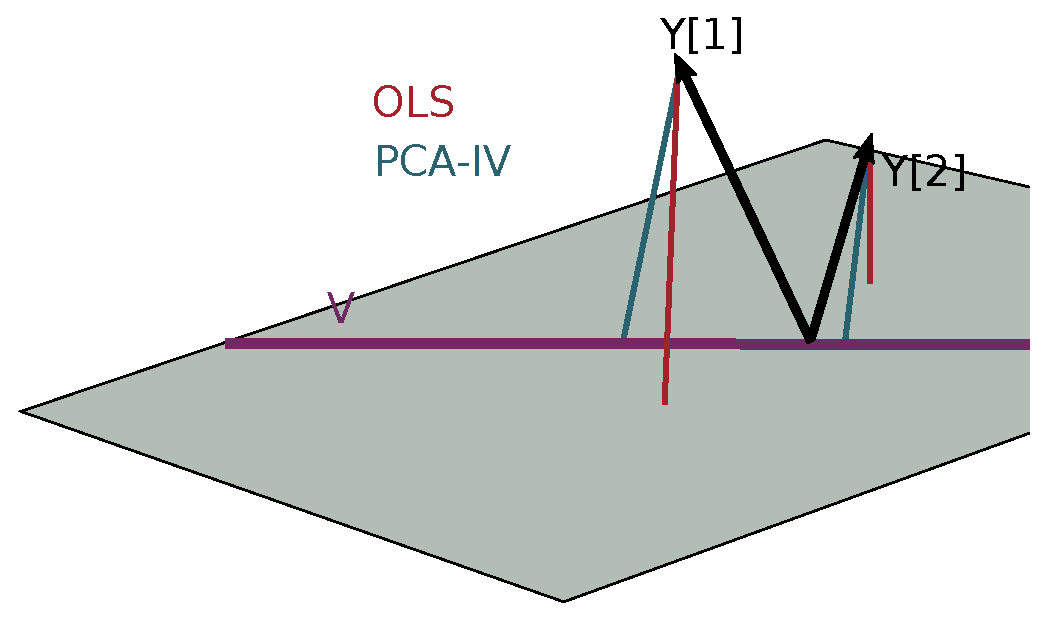
\includegraphics[width=0.7\textwidth]{figure/pca_iv/pca_iv_geometry}
  \caption{A geometric view of PCA-IV. The columns of the response $Y$ are views
    as $n$-dimensional vectors. The grey plane is the span of
    $X$. Multivariate OLS simply projects the columns of $Y$ onto the plane,
    while PCA-IV searches for a further subspace $V$ on which to project all
    responses. \label{fig:pca_iv_geometry} }
\end{figure}

Indeed, write the usual estimates for the covariance matrices of interest,
\begin{align*}
  \hat{\Sigma}_{YY} = \frac{1}{n}Y^{T}Y \\
  \hat{\Sigma}_{YX} = \frac{1}{n}Y^{T}X \\
  \hat{\Sigma}_{XX} = \frac{1}{n}X^{T}X
\end{align*}
and observe that the residual covariance of equation \ref{eq:pca_iv_resid_cov}
can be expressed
\begin{align*}
  &\frac{1}{n}\left[Y^{T}Y -
    Y^{T}XV\left(V^{T}X^{T}XV\right)^{-1}V^{T}X^{T}Y\right] \\
  = &\frac{1}{n}\left[Y^{T}Y^{(T)} - Y^{T}Z\left(Z^{T}Z\right)^{-1}Z^{T}Y\right] \\
  = &Y\left(I - P_{Z}\right)Y,
\end{align*}
where $P_{Z} = Z\left(Z^{T}Z\right)^{-1}Z^{T}$ is the projection operator onto
the columns of $Z$. Minimizing the trace of this matrix is equivalent to
minimizing
\begin{align*}
  \tr\left(Y^{T}\left(I - P_{Z}\right)Y\right) &=
  \tr\left(Y^{T}\left(I - P_{Z}\right)^{T}\left(I -
      P_{Z}\right)Y\right) \\
  &= \|\left(I - P_{Z}\right)Y\|_{F}^{2} \\
  &= \sum_{j = 1}^{p_{1}}\|\left(I - P_{j}\right)y_{\cdot j}\|^{2}_{2},
\end{align*}
which is exactly the sum of squared residuals from the columns of $Y$ onto the
span of the PCA-IV subspace, justifying geometric picture.

\subsubsection{Example}
\label{subsec:pcaiv_example}

Continuing our tour of methods applied to the WELL-China data, we now illustrate
results from PCA-IV. The idea of scores and loadings requires some
clarification. By PCA-IV scores, we mean the coordinates of projections $z_{i}$
of samples onto the subspace defined by $V$, and by loadings, we mean the
correlation between columns\footnote{Geometrically, the angle between original
  columns and the subspace, in the sense of Figure \ref{fig:pca_iv_geometry}.}
of $X$ and $Y$ with the PCA-IV axes defining $V$.

We find that the scores, displayed in Supplementary Figures
\ref{fig:pca_iv_geometry} are similar to those that found by the combined-PCA of
Section \ref{subsec:pca}. One possible explanation for this behavior is that the
PCA-IV generalized SVD of $X$ is similar to an ordinary PCA of $X$, and that in
the combined-PCA of $\left[Y, X\right]$, the fact that $X$ has many more columns
than $Y$ means that the result is similar to a PCA on $X$ alone.

The loadings are given in Figure \ref{fig:pca_iv_loadings}. Interpretation of
the species loadings is simple, since species seem well separated by taxa.
Interpretation of the body composition variables is less clear -- pairs of
variables that would be expected to be near to one another are not, in many
cases. Indeed, \texttt{Trunk\_FM} and \texttt{L\_Total\_FM} would be expected to
have a small angle between one another, but they do not.

\begin{figure}[ht]
  \centering
  \includegraphics[width=\textwidth]{figure/pca_iv/loadings}
  \caption{The loadings for PCA-IV can be interpreted like loadings from
    previous methods. The relationship between variables seems more reasonable
    than in CCA, but are only indirectly related to covariation across
    tables. \label{fig:pca_iv_loadings} }
\end{figure}

\subsection{Partial Triadic Analysis}
\label{subsec:partial_triadic_analysis}

Partial Triadic Analysis (PTA) gives an approach to working with multitable data
when each table has the same dimension \citep{thioulouse2011simultaneous}.
Specifically, it gives a way of analyzing data of the form $\left(X_{\cdot\cdot
  l}\right)_{l = 1}^{L}$, where each $X_{\cdot\cdot l} \in \reals^{n \times p}$;
this is called a data cube because it can also be written as a three-dimensional
array $X \in \reals^{n \times p \times L}$. We denote the $j^{th}$ feature
measured on the $i^{th}$ sample in the $l^{th}$ table by $x_{ijl}$, and the
slices over fixed $i$, $j$, and $l$ by $X_{i \cdot \cdot}$, $X_{\cdot j \cdot}$
and $X_{\cdot \cdot l}$. This type of data arises frequently in longitudinal
data analysis, where the same features are collected for the same samples across
a series of $L$ times. However, the actual ordering of the $L$ tables is not
ever used by this: if we scrambled the time ordering for $L$ tables, the
algorithm's result would not change.

The main idea in PTA is to divide the analysis into two steps,
\begin{itemize}
  \item Combine the $L$ tables into a single compromise table.
  \item Apply any standard single-table method, e.g., PCA, on the
    compromise table.
\end{itemize}

A naive approach to constructing the compromise table would be to average each
entry across the $L$ tables. Instead, PTA upweights tables that are more similar
to the average table, as these are considered more representative. Formally, the
compromise is defined as $X^{(c)} = \sum_{l = 1}^{L}\alpha_{l} X_{\cdot\cdot l}
= X\alpha \in \reals^{n \times p}$, where $\alpha$ (constrained to norm one) is
chosen to maximize $\sum_{l = 1}^{L} \alpha_{l} \left<\overline{X},
X_{\cdot\cdot l}\right>$, a weighted average of inner-products\footnote{We are
  using $\left<A, B\right> = \tr\left(A^{T}B\right)$.} between each of the $L$
tables and the naive-average table, $\overline{X} = \frac{1}{L}\sum_{l = 1}^{L}
X_{\cdot\cdot l}$.

The optimal $\alpha$ can be derived using Lagrange multipliers (see Supplemental
Section \ref{subsec:pta_alpha_derivation}), and leads to the compromise table,
\begin{align*}
  X_{c} = \sum_{l = 1}^{L} \frac{\left<\overline{X}, X_{\cdot\cdot l}\right>}{\sqrt{\sum_{l^{\prime}
      =1}^{L}\left<\overline{X},
      X_{\cdot\cdot l^{\prime}}\right>^{2}}} X_{\cdot\cdot l}.
\end{align*}

We can try to interpret the compromise matrix geometrically. Suppose
the $X_{\cdot\cdot l}$ define an orthonormal basis; so $\left<X^{l},
  X^{l^{\prime}}\right> = \indic{l = l^{\prime}}$. Then, we can write
the compromise table as
\begin{align*}
  X_{c} = \sqrt{L}\sum_{l = 1}^{L}\left<\overline{X},
    X_{\cdot\cdot l}\right>X_{\cdot\cdot l} = \sqrt{L}\overline{X},
\end{align*}
a scaled version of the mean.

If however, the tables are not orthonormal, then we place more weight
on directions that are correlated. For example, if $X^{(1)} =
X^{(2)}$, but the rest of the tables are orthogonal to each other and
to these first two tables, then the compromise double counts the
direction $X^{(1)}$. In this sense, $X_{c}$ is different from the
naive-average $\overline{X}$ -- it upweights more highly
represented tables.

\subsection{Statico and Costatis}
\label{subsec:statico_and_costatis}

In the multivariate ecology literature, it is common to have a pair of data
cubes, giving species abundances and environmental variables over time,
respectively. We write these are $Y \in \reals^{n \times p_{1} \times L}$ and $X
\in \reals^{n \times p_{2} \times L}$. Costatis and Statico are two approaches
for analyzing such data \cite{thioulouse2011simultaneous}. They are easiest to
understand as divide-and-conquer approaches, where the general problem of
analyzing a pair of data cubes is divided into two steps, one designed for analyzing
individual cubes, and another for studying covariation across tables. In Statico, the paired
aspect of the data is dealt with first and followed by a data cube analysis,
while in Costatis, that order is reversed.

Specifically, in Statico, an empirical cross-covariance matrix is constructed at
each time point, $Z^{l} = \frac{1}{n_{l}}Y^{T}_{\cdot\cdot l}X_{\cdot \cdot l}$.
For example, this is, the correlation between the environmental variables and
species counts at a specific timepoint $l$. The $L$ matrices $Z^{(l)}$ are then
input into a PTA, yielding a compromise table $Z_{c}$ which can then be studied
with PCA.

Alternatively, in Costatis, a compromise table is constructed for each of the
data cubes $Y$ and $X$, using PTA. Call these $Y_{c}$ and $X_{c}$. These are now
two matrices each with $n$ rows, and so can be analyzed by any two-table
dimension reduction method. In Costatis, the standard is to apply CoIA to the
pair $Y_{c}, X_{c}$.

Hence, we see that the only difference between these methods is the order
between the CoIA and the PTA. Indeed, this is reflected in the names of the
methods: Statis is an abbreviation for a PTA, and Statico performs a CoIA before
a Statis while Costatis reverses the order.

\subsection{Reduced-rank regression}
\label{subsec:label}

Reduced-rank regression is an approach to multiresponse regression which pools
information across responses \citep{izenman1975reduced, mukherjee2011reduced}.
Compared This pooling can lead to meaningful performance improvements. Further,
we will see that the reduced-rank estimates can aid interpretation as well.

Suppose we have collected $p_{1}$ responses and $p_{2}$ features across $n$
samples, $y_{i} \in \reals^{p_{1}}$ and $x_{i} \in \reals^{p_{2}}$,
respectively. Our goal is to use this training data to predict the response
$y^{\ast}$ given the $x^{\ast}$ from a new sample. Arrange these data into two
matrices, $Y \in \reals^{n \times p_{1}}$ and $X \in \reals^{n \times p_{2}}$.

The simplest approach to this problem is to fit a coefficient matrix $B \in
\reals^{p_{2} \times p_{1}}$ relating the $p_{2}$ features to the $p_{1}$
response coordinates by minimizing $\|Y - XB\|_{F}^{2}$. A slight modification
supposes that the responses might be correlated, and instead optimizes a
whitened version of the problem\footnote{This can also be viewed as using a
  Mahalanobis distance.}, $\|\left(Y -
XB\right)\hat{\Sigma}_{YY}^{-\frac{1}{2}}\|_{F}^{2}$

The optimal $B$ for these two approaches are $\left(X^{T}X\right)^{-1}X^{T}Y$
and $\left(X^{T}\hat{\Sigma}_{YY} X\right)^{-1}X^{T}\hat{\Sigma}_{YY}Y$
respectively. These simply concatenate coefficients from $p_{1}$ independent
(weighted) linear regressions, one per response dimension.

This is not a very satisfactory solution, because we would have hoped to share
information across the different response dimensions: we should be able to
improve performance compared to the univariate regressions. Towards this goal,
consider that while there may be $p_{1}$ responses, their effective dimension
may be relatively low. Reduced-rank regression formalizes this with an explicit
constraint on the rank of $B$, defined by an estimate $\hat{B}^{\text{rr}}$ by
the optimal value of
\begin{align}
\text{minimize}_{B \in \reals^{p_{2} \times p_{1}}} &\|\left(Y - XB\right)\Sigma_{YY}^{-\frac{1}{2}}\|_{F}^{2} \label{eq:rr_obj}\\
\text{such that } &\text{ rank}\left(B\right) \leq K, \nonumber
\end{align}
for some $K < p_{1}\wedge p_{2}$.

The optimal value is given by $\hat{B}^{\text{ols}}V_{K}V_{K}^{-}$, where the
columns of $V_{K}$ are the top $K$ response CCA directions and $V_{K}^{-}$
denotes their pseudoinverse. The derivation is provided in Supplementary Section
\ref{subsec:reduced_rank_derivation}.

Similarly, we can view directly $\hat{Y}^{\text{rr}} = X\hat{B}^{\text{rr}} =
P_{X}YV_{k}V_{k}^{-}$, which means that the reduced-rank fits can be obtained by
first projecting the data columns of $Y$ onto the top $K$ response canonical
directions, and then projecting these pooled $Y$ onto the span of $X$. If the
$Y$ had not been pooled, then the projection onto the span of the $X$'s is
exactly the independent linear regressions approach described above.

\section{Modern multivariate methods}

Compared to classical approaches, modern multivariate methods are typically
designed for more the high-dimensional, heterogeneous settings. The two methods
reviewed in this section are examples of this trend: Partial Least Squares (PLS)
is well-suited for high-dimensional response matrices, while Canonical
Correspondence Analysis (CCpnA) was facilitates joint analysis of the
heterogeneous continuous / count data necessary to answer questions in ecology.
Unlike traditional statistical methods, neither approach is explicitly
model-based, and both are iterative, requiring more extensive computation than
earlier techniques.

\subsection{PLS}
\label{subsec:PLS}

PLS sequentially derives a set of mutually orthogonal features
$\left(z_{k}\right)_{k = 1}^{K}$ that characterizes the relationship between two
tables, $Y$ and $X$ \citep{wold1985partial}. To obtain the first PLS direction,
$z_{1}$, compute the first left singular vector $u_{1}$ of the cross-covariance
matrix between the two tables, $\hat{\Sigma}_{YX} = \frac{1}{n}Y^{T}X$. Then,
for each of the $p_{2}$ columns of $X$, compute the univariate (i.e., partial)
regression coefficient $\hat{\varphi}_{j}$ from the model $u_{1i} = \alpha_{0j}
+ \varphi_{j}x_{ij}$, for $i = 1, \dots, j_{1}$. The first PLS direction is
defined as $z_{1} = X\hat{\varphi}_{1}$. To generate subsequent directions,
orthogonalize both $Y$ and $X$ with respect to the current directions, and
repeat the process.

This procedure is appealing because, like PCA, it reduces a potentially
high-dimensional matrix $X$ with many correlated columns into a
smaller set of orthogonal directions. Moreover, it achieves this
reduction in a way that accounts for correlation with columns in
$Y$: columns of $X$ that are uncorrelated with $Y$
will have no contribution to the PLS directions, even if they account
for a large proportion of variation in $X$.

We have stated the procedure in the form it was originally proposed, but this
algorithmic description is difficult to understand geometrically or
probabilistically. However, statistical interpretations have since been
developed. \citep{frank1993statistical} and \citep{stone1990continuum} studied
the case where $p_{1} = 1$, so $y$ is a single column vector. By assuming that
the rows of $y$ and $X$ are drawn i.i.d. from distributions $\P^{y}$ and
$\P^{X}$, they found that the $k^{th}$ PLS direction $z_{k}$ is the $z$ that
solves the optimization
\begin{align*}
\maximize_{z} & \Corrsubarg{\P^{X} \times \P^{y}}{x_{i}^{T}z_{k},
y_{i}}\Varsubarg{\P^{X}}{z^{T}x_i} \\
\text{such that }&z^{T}y^{T}y z_{j} = 0 \text{ for all }j
\leq k - 1 \text{ and }
\|z\| = 1.
\end{align*}
If the covariance term is omitted, the optimization is identical to the maximum
variance problem that gives the principal component directions based on $X$.
This formulation makes precise the idea that PLS is a version of principal
components that accounts for correlation with $Y$.

An alternative interptetation, due to \citep{gustafsson2001probabilistic}, is
that PLS fits a particular latent variable model. Suppose $\xi_{i} =
\left(\xi_{i}^{s}, \xi_{i}^{X}\right)$ are drawn i.i.d. from a $K_{1} + K_{2} =
K$ dimensional spherical normal. PLS assumes the observed tables $Y$ and $X$
have rows drawn i.i.d. from
\begin{align*}
y_{i} \mid \xi_{i} \sim \Gsn\left(W_{Y}\xi_{i}^{s} +
\mu_{Y}, \sigma^{2}I_{p_{1}}\right) \\
x_{i} \mid \xi_{i} \sim \Gsn\left(W_{X} \xi_{i}^{s} + B_{X}\xi_{i}^{X} +
\mu_{X}, \sigma^{2}I_{p_{2}}\right).
\end{align*}
That is, each table is the sum of two components, one that is a
table-specific linear combination is a shared latent variable, and
another that is an arbitrary linear combination of a table-specific
latent variable. The shared feature $\xi^{s}$ is the object of
interest, and is what PLS implictly estimates.

\subsection{CCpnA}
\label{subsec:canonical-correspondence}

CCpnA is a method, originally developed in ecology, useful for joint analysis of
count and continuous data. The canonical application has a site by species count
matrix $Y \in \reals^{n \times p_{1}}$ and an environmental features matrix $X
\in \reals^{n \times p_{2}}$ (e.g., historical rainfall and temperature
measurements). The scientific goal might be to identify species that are more
abundant in sites with more rainfall or higher temperature. If these
environmental variables were uncorrelated, it would be enough to fit a separate
regression to each; this however is rarely the case, motivating the development
for CCpnA.

CCpnA produces low-dimensional representations for both the rows and columns of
$Y$ (the sites and species), along with latent subspaces on which these
representations are defined. Algorithmically, CCpnA first constructs the
following matrices, where $1_{r}$ denotes a column vector of $r$ ones,
\begin{enumerate}
  \item An overall frequency matrix,
    \begin{align*}
      F = \frac{1}{n_{\cdot\cdot}^{(1)}} Y,
  \end{align*}
  where $n_{\cdot\cdot}^{(1)}$ is the sum of all counts in matrix
  $Y$.
\item A diagonal matrix of row (site) proportions,
  \begin{align*}
    D_{r} &= \diag\left(F 1_{p_{1}}\right) \in \reals^{n \times n}.
  \end{align*}
\item A diagonal matrix of column (species) proportions,
  \begin{align*}
    D_{c} &= \diag\left(F^{T}1_{n}\right) \in \reals^{p_{1} \times p_{1}}.
  \end{align*}
\item A projection onto the columns of the environmental matrix
  $X$, reweighting sites according to their species counts,
  \begin{align*}
    P_{X} &= D_{r}^{\frac{1}{2}}X\left(X^{T}D_{r}X\right)^{-1}X^{T}D_{r}^{\frac{1}{2}} \in
  \reals^{n \times n}.
\end{align*}
\end{enumerate}

With this notation, compute an SVD,
\begin{align*}
D_{r}^{-\frac{1}{2}}\left(F - F 1_{p}1_{p}^{T}F\right)D_{c}^{-\frac{1}{2}}P_{X}
= UDV^{T},
\end{align*}
and define row and column scores $Z$ and $Q$ by
\begin{align*}
  Z &= D_{r}^{-\frac{1}{2}} UD \\
  Q &= D_{c}^{-\frac{1}{2}}V^{T}D.
\end{align*}

There are several ways to interpret this procedure. CCpnA was originally
proposed as the solution to a fixed-point iteration called reciprocal averaging
\citep{ter1986canonical}l. Later, \citep{greenacre1987geometric,
  greenacre1984theory}, provided a geometric view and \cite{zhu2005constrained}
gave an exact probabilistic interpretation.

The intuition for the reciprocal averaging procedure is simple: the
scores for different sites should be a weighted average of the species
scores, with larger weights for the species that are more common at
those sites. That is,
\begin{align*}
  z_{i} \propto \frac{1}{f_{i\cdot}}\sum_{j = 1}^{p_{1}}f_{ij}q_{ij} \\
  q_{j} \propto \frac{1}{f_{\cdot j}} \sum_{i = 1}^{n} f_{ij}z_{ij},
\end{align*}
or, in matrix form,
\begin{align*}
Z \propto \diag\left(F 1_{p}\right)^{-1} F Q^{T} \\
Q \propto \diag\left(F^{T} 1_{n}\right)^{-1} P.
\end{align*}
This formulation suggests a method to obtain $Z$ and $Q$ -- arbitrarily
initialize one and iterate these calculations until convergence.

As is, this is not yet the setup that yields CCpnA\footnote{It in fact gives the
  solution to the Correspondence Analysis problem (the similarity is the reason
  for the name Canonical \textit{Correspondence Analysis}).} -- it doesn't use
information in the environmental table $X$. To recover CCpnA, a projection step
needs to be inserted before the calculation of row scores,
\begin{enumerate}
\item Arbitrarily initialize $Z$.
\item While not converged,
\begin{enumerate}
\item Solve $Q^{\prime} \propto \diag\left(F^{T}1_{n}\right)^{-1}F^{T}Z$.
\item Project $Q = P_{X^{(2)}}Q^{\prime}$.
\item Solve $Z \propto \diag\left(Z 1_{p}\right)^{-1} F Q^{T}$.
\end{enumerate}
\end{enumerate}

The fixed point of this iteration is the previously described CCpnA solution.

A second interpretation, is due to \citep{zhu2005constrained}. Suppose first
that we are only interested in a one-dimensional score for rows and columns. Let
$\alpha$ be a latent environmental gradient, for example, between warm-dry and
cold-wet sites. For each of the $p_{1}$ species, define a normal density over
the environmental variables, $f_{j}\left(x_{i}\right) =
\Gsn_{p^{(2)}}\left(\mu_{j}, \Sigma_{j}\right)$. The mode of this density
represents the preferred environmental conditions for species $j$. Next, project
these densities onto the environmental gradient, giving a univariate
$f_{j}^{\alpha}\left(z_{i}\right) = \Gsn\left(\alpha^{T}\mu_{j}, \alpha^{T}
\Sigma_{j}\alpha\right)$ for each species. The $z_{i}$'s represent the scores
for species $i$ along the environmental gradient $\alpha$.

The generative model views species-site pairs one at a time. For each pair
involving site $i$ and species $j$, draw a score according to
$f_{j}^{\alpha}\left(z_{i}\right)$. That is, for each site $i$, draw a species
according to a $p_{1}$-class LDA model.

To use this idea to compute scores, we need to estimate the environmental
gradient $\alpha$, which is also of interest in its own right. This is done by
supposing equal covariances across species, $\Sigma_{j} = \Sigma$ for all $j$,
and finding the $\hat{\alpha}$ maximizing the between vs. total variance across
species,
\begin{align*}
  \frac{\alpha^{T} \Sigma_{B} \alpha}{\alpha^{T} \Sigma \alpha},
\end{align*}
where
\begin{align*}
  \Sigma_{B} = \sum_{j = 1}^{p_{1}} f_{\cdot j}\left(\mu_{j} -
    \bar{\mu}\right)\left(\mu_{j} - \bar{\mu}\right)^{T}.
\end{align*}
Estimating $\hat{\alpha}$ in this way and writing $z_{i} =
\hat{\alpha}^{T}x_{i}$ gives the original site scores from CCpnA.

\subsection{Kernel CCA}
\label{subsec:kernel_cca}

Since CCA is based on correlation, it can only summarize linear relationships
across tables -- KCCA is a modification that is sensitive to nonlinear
associations \citep{akaho2006kernel, bach2003kernel, lanckriet2004statistical}.
It does this by implicitly lifting the original data to a richer feature space,
with the hope that nonlinear associations in the original data become linear
associations in the richer space -- this is often called the ``kernel trick''
\citep{scholkopf2001kernel}. Informaly, KCCA is the algorithm that emerges after
applying the kernel trick to CCA.

More precisely, let $\varphi^{Y}: \reals^{p_{1}} \to H^{Y}$ and $\varphi^{X}:
\reals^{p_{2}} \to H^{X}$ be mappings from the features directly measured by $X$
and $Y$ into richer spaces $H^{Y}$ and $H^{X}$. For example, the $\varphi$'s
might map vectors into an expansion of all polynomial products of original
feature values, up to some fixed degree (this is mapping is called the
polynomial kernel). As in CCA, let $\P^{X}$ and $\P^{Y}$ denote the sampling
distributions associated with the two tables, and write $x_{i}$ and $y_{i}$ for
generic draws from these distribution.

In the same way that the first CCA direction maximizes the covariance between
linear combinations $u^{T}x_{i}$ and $v^{T}y_{i}$ (subject to a variance
constraint), KCCA maximizes the correlation between the more general inner
products, $z_{i}\left(u\right) = \left<u, x_{i}\right>$ and $z_{i}\left(v\right)
= \left<v, y_{i}\right>$,
\begin{align}
  \argmax_{u \in H^{X}, v \in H^{Y}}
  &\Covsubarg{\P^{X} \times \P^{Y}}{z_{i}\left(u\right), z_{i}\left(v\right)} \label{eq:optim_kcca}\\
\text{subject to } &\Varsubarg{P^{X}}{z_{i}\left(u\right)} = \Varsubarg{P^{Y}}{z_{i}\left(v\right)} = 1. \nonumber
\end{align}

As is, the problem is not well-posed, and it is necessarily to regularize. The
regularized Lagrangian associated with the optimization \ref{eq:optim_kcca} is
\begin{align}
  &\Covsubarg{\P^{X} \times \P^{Y}}{z_{i}\left(u\right), z_{i}\left(v\right)} -
  \frac{\rho^{X}}{2}\Varsubarg{P^{X}}{z_{i}\left(u\right)} -
  \frac{\rho^{Y}}{2}\Varsubarg{P^{Y}}{z_{i}\left(v\right)} + \label{eq:lagrangian_kcca}\\
  &\frac{\lambda^{X}}{2}\text{Pen}\left(u\right) + \frac{\lambda^{(Y)}}{2}\text{Pen}\left(v\right), \nonumber
\end{align}
where $\text{Pen}\left(x\right)$ is some regularizer, the $\ell^{1}$ or
$\ell^{2}$ norm, for example.

The optimal $u$ and $v$ must lie in the spans of
$\left(\varphi^{X}\left(x_{i}\right)\right)_{i =1 }^{n}$ and
$\left(\varphi^{Y}\left(y_{i}\right)\right)_{i =1 }^{n}$, respectively, since
directions orthogonal to these subspaces cannot improve the correlation in the
objective. Therefore,
\begin{align*}
u &= \Phi^{X} \alpha^{X} \\
v &= \Phi^{Y} \alpha^{Y},
\end{align*}
for some $\alpha^{X}, \alpha^{Y}$, where $\Phi^{X} \in \reals^{n \times
  \text{dim}\left(H^{X}\right)}$ has $i^{th}$ row
$\varphi^{Y}\left(x_{i}\right)$ and $\Phi^{Y}$ is defined similarly.

Substituting this into the Lagrangian \ref{eq:lagrangian_kcca}, it becomes clear
that only the cross-products $\Phi^{X T}\Phi^{X}$ and $\Phi^{Y T}\Phi^{Y}$
appear. Since these inner products can be written as kernel matrices -- call
them $K^{X}$ and $K^{Y}$ -- the optimization can be fully expressed in terms of
kernels, without reference to the original $X$ or $Y$. It can then be shown that
the optimal $\alpha^{X}$ and $\alpha^{Y}$ are the solutions to the generalized
eigenvalue problem,
\begin{align*}
  \begin{pmatrix}
    0 & K^{X}K^{Y} \\
    K^{Y}K^{X} & 0
  \end{pmatrix}
  \begin{pmatrix}
    \alpha^{X} \\
    \alpha^{Y}
  \end{pmatrix}
&= \rho
\begin{pmatrix}
  \left(K^{X} + \lambda^{X}I_{p_{1}}\right)^{2} & 0 \\
  0 & \left(K^{Y} + \lambda^{Y}I_{p_{2}}\right)^{2}
\end{pmatrix}
\begin{pmatrix}
  \alpha^{(1)} \\
  \alpha^{(2)}
\end{pmatrix}.
\end{align*}
A geometric interpretation of Kernel CCA was described in
\citep{kuss2003geometry}. The core idea is to translate the Euclidean picture
associated with CCA to the more general RKHS setting. Often, however, KCCA
results can be difficult to study, because only sample scores are provided.
Eigenvectors are never computed in the spaces $H^{X}$ and $H^{Y}$, so it's not
possible to make a biplot. Consequently, KCCA scores are typically interpreted
using supplementary characteristics of the samples.

\subsection{Curds \& Whey}
\label{subsec:cw}

The Curds \& Whey (C\&W) procedure is a ``soft'' version of reduced-rank
regression, differentially shrinking the OLS fits with respect to the response
canonical correlation directions \citep{breiman1997predicting}. This is in
contrast to reduced-rank regression, whose projection onto the first $K$
response canonical correlation directions is the hard-thresholding analog. In
this light, C\&W is to reduced-rank regression what ridge regression is to
principal component regression.

More precisely, the C\&W algorithm fits a table $Y$ according to
\begin{align}
  \hat{Y} &= P_{X}YV\Lambda V^{-1}, \label{eq:cw_yhat}
\end{align}
where again $V \in \reals^{p_{1} \times p_{1}}$ are the CCA directions
associated with the response $Y$ and $P_{X}$ is the projection operator onto the
column space of $X$. $\Lambda$ is defined to be a diagonal matrix the determines
the degree of shrinkage for the different canonical directions.

The main difficulty in C\&W is the choice of $\Lambda$, and
\citep{breiman1997predicting} provide several options. One nice choice can be
derived from a generalized cross-validation point of view. It turns out that
shrinkage towards the response canonical correlation directions emerges
automatically, without assuming the form \ref{eq:cw_yhat} a priori. This
derivation is provided in Supplementary Section
\ref{subsec:derivation_curds_and_whey}.

\bibliographystyle{plainnat}
\bibliography{refs.bib}

\section{Appendix}

\subsection{Additional figures}

\begin{figure}
  \includegraphics[width=0.7\textwidth]{figure/pca/proj_plot_2}
  \caption{This is the analog of Figure \ref{fig:pca-approx} in the case that
    PCA is run on all body composition variables, rather than just  and
    Fatmass. That is, we project the original values for these two features
    onto the top two PCs obtained from a PCA on all body composition variables.
    Since the PCA is working in a large space, the projected points are
    generally not too far from their original positions. However, note that one
    outlier on the far right is projected into the bulk of points in the center
    -- the variation coming from this one point is too specific to be preserved
    by PCA.
  \label{fig:pca-approx-2}}
\end{figure}

\begin{figure}
  \includegraphics[width=0.7\textwidth]{figure/pca/proj_plot_3}
  \caption{Here we perform the same procedure as in Figure
    \ref{fig:pca-approx-2}, except instead of projecting onto the top two PCs,
    we project onto only the top PC. The main point is that, while in two
    dimensions (Figure \ref{fig:pca-approx}), the behavior of the projection is
    easy to understand in terms of orthogonal errors, the corresponding
    orthogonal projection in higher dimensions is more complex.
  \label{fig:pca-approx-3}}
\end{figure}

\begin{figure}[ht]
  \centering \includegraphics[width=\textwidth]{figure/coia/loadings}
  \caption{These are the loadings obtained from CoIA, which are analogous to
    those obtained from concatenated PCA (Figure \ref{fig:loadings}) and CCA
    (Figure \ref{fig:cca_loadings}). \label{fig:coia_loadings} }
\end{figure}

\begin{figure}[ht]
  \centering
  \includegraphics[width=\textwidth]{figure/coia/scores_rl_ratio}
  \caption{These the same CoIA scores as in Figure \ref{fig:coia_scores_total_fm},
    but shaded instead by Ruminococcaceae / Lachnospiraceae ratio, as in Figures
    \ref{fig:scores_rl_ratio} and
    \ref{fig:cca_scores_rl_ratio}. \label{fig:coia_scores_rl_ratio} }
\end{figure}

\begin{figure}[ht]
  \centering
  \includegraphics[width=\textwidth]{figure/pca_iv/scores_total_fm}
  \caption{We can display the scores obtained by PCA-IV. The results are similar
    to those from combined-PCA, which is not surprising, since they are related
    to the PCA based only on microbial
    abundances. \label{fig:pca_iv_scores_total_fm} }
\end{figure}

\begin{figure}[ht]
  \centering
  \includegraphics[width=\textwidth]{figure/pca_iv/scores_rl_ratio}
  \caption{This provides the same scores as Figure
    \ref{fig:pca_iv_scores_total_fm}, but shaded by Ruminoccoccaceae vs.
    Lachnospiraceae ratio. \label{fig:pca_iv_scores_rl_ratio} }
\end{figure}

\subsection{Derivation details for PCA-IV}
\label{subsec:pca_iv_derivation}

In this section, we provide the argument for why the generalized
eigendecomposition $\hat{\Sigma}_{XY}\hat{\Sigma}_{YX} =
\hat{\Sigma}_{XX}V\Lambda V^{T}$ provides the optimal $V$ used in PCA-IV.

First consider $k = 1$. Then, for any $\tilde{v}$, the objective
\ref{eq:pca_iv_obj_2} has the form
\begin{align}
  \tr\left(\hat{\Sigma}_{YX}\tilde{v}\left(\tilde{v}\hat{\Sigma}_{XX}\tilde{v}\right)^{-1}
  \left(\hat{\Sigma}_{YX}\tilde{v}\right)^{T}\right) &=
  \frac{\tilde{v}^{T}\Sigma_{XY}\Sigma_{YX}\tilde{v}}{\tilde{v}^{T}\Sigma_{XX}\tilde{v}} \label{eq:gev_opt_1}\\
  &= \frac{\tilde{w}^{T}\Sigma_{XX}^{-\frac{1}{2}}\Sigma_{XY}\Sigma_{YX}\Sigma_{XX}^{-\frac{1}{2}}\tilde{w}}{\|\tilde{w}\|_{2}^{2}}, \label{eq:gev_opt_2}
\end{align}
where we change variables $\tilde{w} = \Sigma_{XX}^{\frac{1}{2}}\tilde{v}$. But
to maximize \ref{eq:gev_opt_2}, just choose $\tilde{w}$ to be the top
eigenvector of
$\Sigma_{XX}^{-\frac{1}{2}}\Sigma_{XY}\Sigma_{YX}\Sigma_{XX}^{-\frac{1}{2}}$,
which implies that $\tilde{v}$ is the top generalized eigenvector of
$\Sigma_{XY}\Sigma_{YX}$ with respect to $\Sigma_{XX}$. Indeed, in this case,
\begin{align*}
  \Sigma_{XY}\Sigma_{YX}\tilde{v}
  &=\Sigma_{XY}\Sigma_{YX}\Sigma_{XX}^{-\frac{1}{2}}\tilde{w} \\
  &= \Sigma_{XX}^{\frac{1}{2}} \Sigma_{XX}^{-\frac{1}{2}}\Sigma_{XY}\Sigma_{YX} \Sigma_{XX}^{-\frac{1}{2}}\tilde{w}\\
  &= \Sigma_{XX}^{\frac{1}{2}}\lambda_{1}\tilde{w} \\
  &= \lambda_{1}\Sigma_{XX}\tilde{v}.
\end{align*}

Hence, in the case $K = 1$, the criterion is maximized by the top generalized
eigenvector. For larger $K$, recall that the problem of maximizing
$\frac{v^{T}Av}{\|v\|^{2}}$ over $v$ subject to being orthogonal to the first $K
- 1$ eigenvectors of $A$ is solved by the $K^{th}$ eigenvector of $A$, and
applying this fact in step \ref{eq:gev_opt_2} of the argument above gives the
result for general $K$.

\subsection{Derivation of PTA $\alpha$}
\label{subsec:pta_alpha_derivation}

 The Lagrangian of the optimization defined by PTA is
\begin{align*}
\mathcal{L}\left(\alpha, \lambda\right) &= \sum_{l = 1}^{L}
\alpha_{l}\left<\overline{X}, X_{\cdot\cdot l}\right> +
\lambda\left(\|\alpha\|^{2}_{2} - 1\right),
\end{align*}
which when differentiated with respect to $\alpha$ yields $\alpha_{l} =
-\frac{1}{2\lambda} \left<\overline{X}, X_{\cdot\cdot l}\right>$ for all $l$.
The constraint that $\|\alpha\|_{2}^{2} = 1$ implies that
$\frac{1}{4\lambda^{2}} \sum_{l^{\prime} = 1}^{L} \left<\overline{X},
X_{\cdot\cdot l^{\prime}}\right>^{2} = 1$, which gives $\lambda = \frac{1}{2}
\sqrt{\sum_{l^{\prime} =1 }^{L} \left<\overline{X}, X_{\cdot\cdot
    l^{\prime}}\right>^{2}}$, so $\alpha_{l} = \frac{\left<\overline{X},
  X_{\cdot\cdot l}\right>}{\sqrt{\sum_{l^{\prime} =1}^{L}\left<\overline{X},
    X_{\cdot\cdot l^{\prime}}\right>^{2}}}$.

\subsection{Derivation of Reduced Rank Solution}
\label{subsec:reduced_rank_derivation}

Consider the data and parameters in the whitened space, $Y^{\ast} =
Y\hat{\Sigma}_{YY}^{-\frac{1}{2}}$ and $B^{\ast} =
B\hat{\Sigma}_{YY}^{-\frac{1}{2}}$, and rewrite the objective \ref{eq:rr_obj} as
\begin{align*}
\|Y^{\ast} - XB^{\ast}\|_{F}^{2} &= \|Y^{\ast} - \hat{Y}^{\ast \text{ols}}\|_{F}^{2} + \|\hat{Y}^{\ast \text{ols}} - XB^{\ast}\|_{F}^{2},
\end{align*}
where we used the fact that the residuals are orthogonal to the column space of
$X$ to remove the cross term. The first term does not involve $B^{\ast}$, so we
can focus on minimizing the second. Consider the SVD $\hat{Y}^{\ast \text{ols}}
= \dot{U}\dot{D}\dot{V}^{T}$. We know that the matrix $A$ of rank $K$ that
minimizes $\|\hat{Y}^{\ast \text{ols}} - A\|_{F}^{2}$ is $A =
\dot{U}_{K}\dot{D}_{K}\dot{V}_{K}^{T} = Y^{\ast
  \text{ols}}\dot{V}_{k}\dot{V}_{k}^{T}$, the truncated SVD of $\hat{Y}^{\ast
  \text{ols}}$, or alternatively its projection onto the top $K$ right
eigenvectors.

In particular, any matrix $B$ that satisfies
\begin{align*}
  XB^{\ast} = \hat{Y}^{\ast \text{ols}}\dot{V}_{k}\dot{V}_{k}^{T} = X\hat{B}^{\ast \text{ols}}\dot{V}_{k}\dot{V}_{k}^{T}
\end{align*}
solves the reduced rank regression problem, so we can choose
\begin{align}
  \hat{B}^{\text{rr}} &= \hat{B}^{\ast \text{ols}}\dot{V}_{k}\dot{V}_{k}^{T}, \label{eq:brr_coef}
\end{align}
which involves $\hat{B}^{\ast \text{ols}}$, the OLS fit of $Y^{\ast}$ on $X$, and
$V_{k}$, the top $K$ right eigenvectors of the resulting fitted vector
$\hat{Y}^{\ast \text{ols}}$.

There is a connection between this fit and the response canonical directions of
$\hat{Y}$. In particular, consider the eigendecomposition that follows from the
earlier SVD,
\begin{align}
\dot{V}\dot{D}\dot{V}^{T} &=   \hat{Y}^{\ast \text{ols} T}  \hat{Y}^{\ast \text{ols}} \nonumber \\
&= \left(P_{X}Y\Sigma_{YY}^{-\frac{1}{2}}\right)^{T}\left(P_{X}Y\Sigma_{YY}^{-\frac{1}{2}}\right)\nonumber \\
  &= \Sigma_{YY}^{-\frac{1}{2}}\Sigma_{YX} \Sigma_{XX}^{-1}\Sigma_{XY}\Sigma_{YY}^{-\frac{1}{2}}. \label{eq:star_ols}
\end{align}

Recall that the response canonical directions $V$ are derived by taking the SVD
of $\Sigma_{XX}^{-\frac{1}{2}}\Sigma_{XY}\Sigma_{YY}^{-\frac{1}{2}} =
\tilde{U}\tilde{D}\tilde{V}^{T}$ and setting $V =
\Sigma_{YY}^{-\frac{1}{2}}\tilde{V}$. But comparing this to the form of Equation
\ref{eq:star_ols}, we find that $\dot{V} = \tilde{V}$, the eigenvectors from
which the CCA response directions are derived are equal to the eigenvectors of
the cross-products of the OLS fits in the whitened space. Hence,
\begin{align*}
\hat{B}^{\text{rr}} &= \hat{B}^{\ast \text{ols}}\tilde{V}_{K}\tilde{V}_{K}^{T} \\
&= \left(X^{T}X\right)^{-1}X^{T}Y^{\ast}\tilde{V}_{K}\tilde{V}_{K}^{T} \\
&= \left(X^{T}X\right)^{-1}X^{T}Y\Sigma_{YY}^{-\frac{1}{2}}\tilde{V}_{K}\tilde{V}_{K}^{T} \\
&= \left(X^{T}X\right)^{-1}X^{T}Y V_{K} \Sigma_{YY}^{\frac{1}{2}}V_{K}^{T} \\
&= \hat{B}^{\text{ols}}V_{K}V_{K}^{-},
\end{align*}

Therefore, the reduced-rank coefficients are just the projection of the original
OLS coefficients onto the subspace spanned by the top $K$ response canonical
directions.

\subsection{Derivation of Curds \& Whey Shrinkage}
\label{subsec:derivation_curds_and_whey}

Consider prediction across many related response variables. One way to pool
information across respones is to define new fitted values from a linear
combination of independent OLS fits. That is, to predict a response $y_{i} \in
\reals^{p_{1}}$, we set $\hat{y}^{\text{cw}}_{i} = B\hat{y}^{\text{ols}}_{i}$
for some square matrix $B \in \reals^{p_{1} \times p_{1}}$. But how to choose
$B$? One reasonable idea is to choose a $B$ that has the best performance in a
full leave-one-out cross-validation (LOOCV),
\begin{align}
  \hat{B}^{\text{cw}} := \arg\min_{B} \sum_{i = 1}^{n} \|y_{i} - B \hat{y}_{-i}\|_{2}^{2}. \label{eq:cv_looc}
\end{align}

Here, $\hat{y}_{-i}$ is the OLS fitted value for $y_{i}$ when training on all
samples but the $i^{th}$. For ease of notation, we write $\hat{y}$ instead of
$\hat{y}^{\text{ols}}$, referring explicitly to $\hat{y}^{\text{c\&w}}$ when
needed.

It is well known that $\hat{y}_{-i}$ can be decomposed as
\begin{align}
  \hat{y}_{-i} &= \left(1 - g_{i}\right)y_{i} + g_{i} \hat{y}_{i}, \label{eq:cv_looc_trick}
\end{align}
where $g_{i} = \frac{1}{1 - h_{ii}}$ and $h_{ii}$ are the diagonal elements of
the projection matrix $P_{X}$ and $\hat{y}_{i}$ is the fitted value on the
$i^{th}$ sample, both computed using all the data (see for example
\citep{seber2012linear}).

The advantage of the representation \ref{eq:cv_looc_trick} is that it makes it
possible to perform LOOCV without computing $n$ regression models: from a single
full regression using all the data, all the LOOCV fits $\hat{y}_{-i}$ can be
deduced directly. This can dramatically speed up computation of the sum in
\ref{eq:cv_looc}.

An alternative is to use generalized cross-validation (GCV). This
approach suggests a form for $B$ based on the response canonical
correlation directions. The GCV approximation is that the $h_{ii}$ can
be approximated by their average across all diagonal elements of $H$:
$h_{ii} \approx h := \frac{1}{n}\tr\left(H\right)$ for all $i$. In
this spirit, define $g = \frac{1}{1 - h}$, and approximate
\begin{align*}
  \hat{y}_{-i} \approx \left(1 - g\right)y_{i} + g\hat{y}_{i}.
\end{align*}

Then, the LOOCV error optimized in \ref{eq:cv_looc} can be simplified to
\begin{align}
  \sum_{i = 1}^{n}\|y_{i} - B\hat{y}_{-i}\|_{2}^{2} &= \sum_{i =
    1}^{n} \|y_{i} - B\left(\left(1 - g\right)y_{i} +
    g\hat{y}_{-i}\right)\|_{2}^{2},
\end{align}
and differentiating with respect to $B$, we find that the optimal
$\hat{B}^{\text{cw}}$ in this GCV framework must satisfy
\begin{align}
\sum_{i = 1}^{n}\left(y_{i} - B\left(\left(1 - g\right)y_{i} +
    g\hat{y}_{-i}\right)\right)\left(\left(1 - g\right)y_{i} +
  g\hat{y}_{-i}\right)^{T},
\end{align}
or equivalently
\begin{align}
\sum_{i = 1}^{n} y_{i}\left(\left(1 - g\right)y_{i} +
  g\hat{y}_{-i}\right)^{T} &=  \sum_{i = 1}^{n}B\left(\left(1 -
    g\right)y_{i} + g\hat{y}_{-i}\right)\left(\left(1 - g\right)y_{i}
  +  g\hat{y}_{-i}\right)^{T},
\end{align}
which in matrix form is
\begin{align}
\left(1 - g\right)Y^{T}Y + g\hat{Y}^{T}Y = B\left(\left(1 - g\right)Y
  + g \hat{Y}\right)^{T}\left(\left(1 - g\right)Y + g \hat{Y}\right), \label{eq:gcv_mat_form}
\end{align}
where $\hat{Y} \in \reals^{n \times p_{1}}$ has $i^{th}$ row
$\hat{y}_{-i}$.

Now, we can represent these cross-products in a way that is suggestive
of CCA,
\begin{align}
  Y^{T}Y &= n \hat{\Sigma}_{YY} \\
  \hat{Y}^{T}Y &= Y^{T}HY = Y^{T}X\left(X^{T}X\right)^{-1}X^{T}Y =
  n\hat{\Sigma}_{YX}\hat{\Sigma}_{XX}^{-1} \hat{\Sigma}_{XY} \\
  \hat{Y}^{T}\hat{Y} &= Y^{T}P_{X}^2 Y = Y^{T}P_{X}Y=
  n\hat{\Sigma}_{YX}\hat{\Sigma}_{XX}^{-1} \hat{\Sigma}_{XY},
\end{align}
Substituting this notation into \ref{eq:gcv_mat_form} and
ignoring the scaling $n$ yields
\begin{align}
\left(1 - g\right)\hat{\Sigma}_{YY} + g
\hat{\Sigma}_{YX}\hat{\Sigma}_{XX}^{-1}\hat{\Sigma}_{XY} &=
B\left[\left(1 - g\right)\hat{\Sigma}_{YY} + \left(2g -
    g^{2}\right)\hat{\Sigma}_{YX}\hat{\Sigma}_{XX}^{-1}\hat{\Sigma}_{XY}\right].
\end{align}
Postmultiplying by $\hat{\Sigma}_{YY}$ gives
\begin{align}
  \left(1 - g\right)I_{p_{1}} + g\hat{Q}^{T} &= B\left[\left(1 -
      g\right)I_{p_{1}} + \left(2g -
      g^{2}\right)\hat{Q}^{T}\right], \label{eq:cca_gcv_id}
\end{align}
where,
\begin{align}
\hat{Q} :=
\hat{\Sigma}_{YY}^{-1}\hat{\Sigma}_{YX}\hat{\Sigma}_{XX}^{-1}\hat{\Sigma}_{XY}
\in \reals^{p_{1}\times p_{1}}.
\end{align}
Now, we claim that we can decompose $\hat{Q} = VD^{2}V^{-1}$, where $V
\in \reals^{p_{1} \times p_{1}}$ is the full matrix of CCA response
directions and  $D$ is diagonal with the canonical correlations. Indeed,
the usual CCA response directions $V$ can be recovered by setting $V =
\hat{\Sigma}_{YY}^{-\frac{1}{2}}\tilde{V}$, where $\tilde{V}$ comes
from the SVD of $A :=
\Sigma_{XX}^{-\frac{1}{2}}\Sigma_{XY}\Sigma_{XX}^{-\frac{1}{2}} =
\tilde{U}D\tilde{V}^{T}$. We then note that
\begin{align}
  Q &= \Sigma_{YY}^{-\frac{1}{2}}A^{T}A\Sigma_{YY}^{\frac{1}{2}} \\
  &=
  \Sigma_{YY}^{-\frac{1}{2}}\tilde{V}^{2}D^{2}\tilde{V}^{T}\Sigma_{YY}^{\frac{1}{2}}\\
  &= VD^{2}V^{-1},
\end{align}
where we are able to write $V^{-1} =
\tilde{V}^{T}\Sigma_{YY}^{\frac{1}{2}}$ because $\tilde{V}$ is the
full (untruncated) matrix of eigenvectors, so $\tilde{V}\tilde{V}^{T}
= I$ in addition to the usual $\tilde{V}^{T}\tilde{V} =I$, which holds
even for the truncated SVD.

Therefore, \ref{eq:cca_gcv_id} can be expressed as
\begin{align}
  V^{-T}\left[\left(1 - g\right)I_{p_{1}} + gD^{2}\right]V^{T} &=
  BV^{-T}\left[\left(1 - g\right)I_{p_{1}} + \left(2g -
      g^2\right)D^{2}\right]V^{T}
\end{align}
so, the $B$ satisfying the normal equations has the form
\begin{align}
\hat{B}^{\text{cw}} &= V^{-T}\Lambda V^{T},
\end{align}
where $\Lambda$ is a diagonal matrix with entries
\begin{align}
\lambda_{jj} = \frac{1 - g + d_{jj}^{2}g}{1 - g + \left(2g -
    g^{2}\right)d_{jj}^{2}}.
\end{align}
Notice that when $n$ is large, $\frac{1}{n}\tr P_{X}$ will be small,
so $g \approx 0$ and less shrinkage will be applied.

Recall that $\hat{B}^{\text{cw}}$ is used to pool across OLS fits,
$\hat{y}_{i}^{\text{cw}} = \hat{B}^{\text{cw}}\hat{y}_{i}^{\text{ols}}$. That is,
\begin{align}
\hat{Y}^{\text{cw}} &= \hat{Y}^{\text{ols}}B^{T} =
\hat{Y}^{\text{ols}}V\Lambda V^{-1}
\end{align}
which we can also view as $\hat{Y}^{\text{cw}}V =
\left(\hat{Y}^{\text{ols}}V\right)\Lambda$. This means that the
C\&W coordinates along the canonical directions $V$ are set as the OLS
fits $\hat{Y}^{\text{ols}}$ along the canonical directions $V$, with
weights defined by $\Lambda$. The actual $\hat{Y}^{\text{cw}}$ are
recovered by transforming back to the original coordinate system. A
similar way to view the C\&W fits is $\hat{Y}^{\text{cw}}V =
P_{X}\left(YV\right)\Lambda$. From this point of view, we shrink the
original data $Y$ according to the canonical directions, and then
project the shrunk data onto the subspace defined by the columns of
$X$. In any case, we see that C\&W pools across regression problems
through a soft shrinkage weighted along canonical response
directions.


\end{document}
